\documentclass[conference]{IEEEtran}

%% Packages
\usepackage{amsmath,amssymb,amsfonts}
\usepackage{cite}
\usepackage{graphicx}
\usepackage{xcolor}
\usepackage{hyperref}
\usepackage{booktabs}
\usepackage{tabularx}

\def\BibTeX{{\rm B\kern-.05em{\sc i\kern-.025em b}\kern-.08em
    T\kern-.1667em\lower.7ex\hbox{E}\kern-.125emX}}

%% Colors
\definecolor{link-blue}{RGB}{30,120,210}
\definecolor{link-burgundy}{RGB}{140,30,50}

%% PDF document properties + colored hyperlinks (citations blue, cross-references burgundy)
\hypersetup{
  pdfauthor={Mathis Delsart, Achille Morenville, \'Eric Piette},
  pdftitle={Combining Spatial and Entity-Based Reasoning for Competitive MicroRTS Via U-Net and Transformers},
  pdfsubject={Deep Reinforcement Learning for Competitive Agents in MicroRTS: Architecture, Training, and Tournament Evaluation},
  pdfkeywords={Deep Reinforcement Learning, Real-Time Strategy Games, MicroRTS, Entity-Based Reasoning, Spatial Reasoning, U-Net, Transformer},
  colorlinks=true,
  urlcolor=link-blue,
  linkcolor=link-burgundy,
  citecolor=link-blue
}

%% Commands
\newcommand{\code}[1]{{\ttfamily\hyphenchar\font=45\relax #1}}
\newcommand{\urlref}[2]{\href{#1}{\textcolor{black}{#2}}}

%% Document
\begin{document}

% Title + authors
\title{Combining Spatial and Entity-Based Reasoning for Competitive MicroRTS via U-Net and Transformers}

\author{%
  \IEEEauthorblockN{Mathis Delsart}
  \IEEEauthorblockA{\textit{ICTEAM, UCLouvain} \\
                    Louvain-la-Neuve, Belgium}
  \and
  \IEEEauthorblockN{Achille Morenville}
  \IEEEauthorblockA{\textit{ICTEAM, UCLouvain} \\
                    Louvain-la-Neuve, Belgium}
  \and
  \IEEEauthorblockN{Éric Piette}
  \IEEEauthorblockA{\textit{ICTEAM, UCLouvain} \\
                    Louvain-la-Neuve, Belgium}%
}

% 2026 Copyright Notice
\IEEEoverridecommandlockouts
\IEEEpubid{\makebox[\columnwidth]{979-8-3315-9476-3/26/\$31.00 \copyright2026 IEEE\hfill}
\hspace{\columnsep}\makebox[\columnwidth]{ }}

\maketitle

\IEEEpubidadjcol

\begin{abstract}
In MicroRTS, a real-time strategy benchmark, winning requires long-range coordination between many units. Yet, current deep reinforcement learning agents reason only over spatial feature maps and treat units implicitly through stacks of channels. The contributions of this paper are twofold: \textbf{\emph{(i)}} \code{UECD}, a hybrid architecture coupling spatial and per-unit reasoning explicitly via a multi-scale convolutional backbone and a Transformer over unit entities; and \textbf{\emph{(ii)}} a PPO-based training recipe derived from systematic ablation. On the \emph{basesWorkers16x16A} map, \code{UECD} outranks prior competition winners, topping an open-source and reproducible tournament with a $96.67$\% win rate.
\end{abstract}

\begin{IEEEkeywords}
Deep Reinforcement Learning, Real-Time Strategy Games, MicroRTS, Entity-Based Reasoning, Spatial Reasoning, U-Net, Transformer
\end{IEEEkeywords}

\section{Introduction}

Real-time strategy (RTS) games combine large combinatorial action spaces, multi-unit coordination, sparse long-horizon rewards, and real-time constraints, making them a challenging benchmark for sequential decision-making~\cite{buroRTSChallenge2003, ontanonSurveyRealTimeStrategy2013}. AlphaStar~\cite{vinyalsGrandmasterLevelStarCraft2019} demonstrated Grandmaster-level play in StarCraft~II through deep reinforcement learning (DRL), but at an extreme compute cost ($384$ TPUs over $44$ days). MicroRTS~\cite{ontanonCombinatorialMultiArmedBandit2013} distills RTS gameplay onto small grid maps while preserving its core difficulties and has served as the IEEE Conference on Games (CoG) MicroRTS competition benchmark since $2017$~\cite{ontanonFirstMicroRTSArtificial2018}. Current MicroRTS agents fall into two paradigms: DRL agents such as \urlref{https://github.com/sgoodfriend/rl-algo-impls}{RAISocketAI}~\cite{goodfriendCompetitionWinningDeep2024}, dominant on small maps ($\le\!16{\times}16$) where per-tick inference cost remains manageable, and rule-based bots such as \urlref{https://github.com/Coac/coac-ai-microrts}{CoacAI}, \urlref{https://github.com/barvazkrav/mayariBot}{Mayari}, \urlref{https://github.com/Jannis42/MicroRTSObiBotKenobi}{ObiBotKenobi}, and \urlref{https://github.com/MazzaAlessandro/TMA}{TMA}, which generalize to larger layouts within tight time budgets.

Purely convolutional backbones capture long-range unit interactions only indirectly. This paper addresses this limitation through two contributions: \textbf{\emph{(i)} \code{UECD}}, a hybrid architecture combining a multi-scale encoder-decoder with skip connections (U-Net)~\cite{ronnebergerUNetConvolutionalNetworks2015} gated by channel-and-spatial attention (CBAM, Convolutional Block Attention Module)~\cite{wooCBAMConvolutionalBlock2018} for spatial reasoning, and an entity Transformer~\cite{vaswaniAttentionAllYou2017} for unit-level reasoning; and \textbf{\emph{(ii)} a PPO-based training recipe}~\cite{schulmanProximalPolicyOptimization2017} derived from systematic ablation, introducing \emph{Matchup Competitiveness Weighting} and two-phase opponent-pool fine-tuning.

\code{UECD} is benchmarked in an open-source, reproducible tournament prompted by the 2026 CoG MicroRTS competition's shift to Large Language Model (LLM) agents. On the \emph{basesWorkers16x16A} map, \code{UECD} tops the standings against past CoG winners and baselines, achieving a $96.67$\% win rate (WR) and a $9$--$1$ head-to-head record against RAISocketAI. Robustness is further evaluated under layout and scale shifts.

\section{Background and Related Work}
\label{sec:background}

MicroRTS-Py~\cite{huangGym$m$RTSAffordableFull2021} exposes MicroRTS as an RL environment. Its \urlref{https://github.com/Farama-Foundation/MicroRTS-Py}{GridNet} PPO baseline, using per-cell action logits with invalid-action masking~\cite{huangCloserLookInvalid2022}, reaches $91\%$ WR on \emph{basesWorkers16x16A} as Player~$0$ (P0) against a $2021$-era pool. Building on this framework, RAISocketAI~\cite{goodfriendCompetitionWinningDeep2024}, the strongest published DRL agent for MicroRTS, trains a $5$\,M-parameter backbone via self-play and a fixed opponent pool; several design choices inform the ablations in Section~\ref{sec:experiments}.

AlphaStar~\cite{vinyalsGrandmasterLevelStarCraft2019} introduced two ideas adopted here: \emph{per-unit Transformer encoding}, which represents units as discrete entities rather than as pixels in a feature map; and \emph{Prioritized Fictitious Self-Play} (PFSP), which samples opponents from a historical league weighted by matchup difficulty.

Further details on competition rules, mechanics, and the environment are available in~\cite{ontanonFirstMicroRTSArtificial2018,huangGym$m$RTSAffordableFull2021} and the project \href{https://github.com/Farama-Foundation/MicroRTS/wiki/Game-Definition}{\textcolor{link-blue}{Wiki}}.

\section{UECD Architecture}
\label{sec:arch}

Fig.~\ref{fig:cbam-deep-arch} shows the proposed \code{UECD} architecture, short for \code{U-Net-Entity-CBAM-Deep}. Unlike purely spatial baselines, \code{UECD} combines three complementary reasoning axes:

\begin{figure*}[!bt]
    \centering
    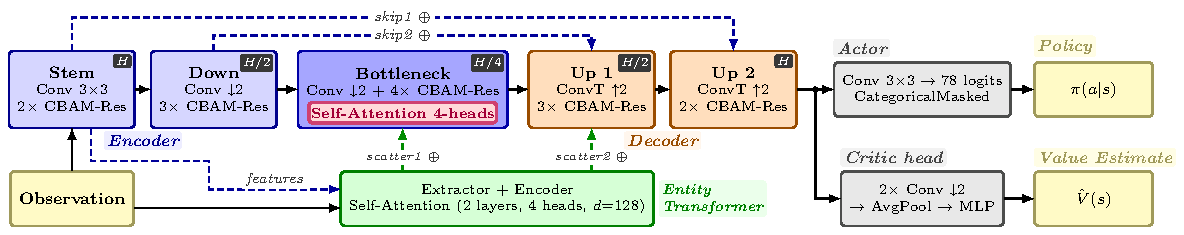
\includegraphics[width=\textwidth]{figures/arch_cbam_deep.pdf}
    \caption{\textbf{\code{UECD} Architecture:} CBAM-gated U-Net encoder-decoder (blue/orange) with bottleneck self-attention (red) and a parallel Entity Transformer (green), scattering enriched features at two scales. Actor and critic heads (gray) produce policy logits $\pi(a|s)$ and value estimates $\hat{V}(s)$ from the observation (yellow).}
    \label{fig:cbam-deep-arch}
\end{figure*}

\paragraph*{\textbf{1. Spatial perception}}
A CBAM-gated U-Net~\cite{ronnebergerUNetConvolutionalNetworks2015,wooCBAMConvolutionalBlock2018} backbone (Fig.~\ref{fig:cbam-deep-arch}, blue and orange) performs multi-scale spatial reasoning through skip connections between the encoder and decoder. Unlike channel-only Squeeze-and-Excitation (SE) attention~\cite{huSqueezeandExcitationNetworks2018}, CBAM jointly weights channels and spatial regions (e.g. HP channels and frontlines). Most depth sits at the bottleneck, where small feature maps keep it cheap.

\paragraph*{\textbf{2. Relational reasoning}}
A parallel Entity Transformer~\cite{vaswaniAttentionAllYou2017} (Fig.~\ref{fig:cbam-deep-arch}, green) captures long-range unit interactions explicitly (e.g. units coordinating an attack). Each unit is encoded as a token combining raw attributes, spatial features, and positional embeddings. Refined entity features are scattered additively back into the spatial map at both bottleneck (strategic) and mid-resolution (tactical) scales.

\paragraph*{\textbf{3. Global spatial reasoning}}
A lightweight 4-head self-attention layer over the bottleneck grid (Fig.~\ref{fig:cbam-deep-arch}, red) captures long-range region-to-region dependencies beyond local convolutional receptive fields (e.g. front push vs.\ base defense).

\section{Setup and Methodology}
\label{sec:setup-method}

Training runs on the standard $16{\times}16$ \emph{basesWorkers16x16A} map ($4000$-step episode cap), across $24$ parallel bot environments ($9$ CoacAI, $9$ Mayari, $2$ \urlref{https://github.com/Farama-Foundation/MicroRTS/blob/master/src/ai/RandomBiasedAI.java}{RandomBiasedAI}, $2$ \urlref{https://github.com/Farama-Foundation/MicroRTS/blob/master/src/ai/abstraction/partialobservability/POWorkerRush.java}{POWorkerRush}, $2$ \urlref{https://github.com/Farama-Foundation/MicroRTS/blob/master/src/ai/abstraction/partialobservability/POLightRush.java}{POLightRush}; sides swapped per episode). PPO~\cite{schulmanProximalPolicyOptimization2017} with Generalized Advantage Estimation (GAE)~\cite{schulmanHighDimensionalContinuousControl2015} uses $\gamma{=}0.99$, $\lambda_{\text{GAE}}{=}0.95$, $\epsilon_{\text{clip}}{=}0.1$, rollouts/epochs/minibatches $=512/2/3$, $c_v{=}0.5$, max grad norm $0.5$; learning rate and entropy linearly annealed from $2.5e{-}4{\to}0$ and $1e{-}2{\to}1e{-}3$, respectively. Reward weights follow~\cite{huangGym$m$RTSAffordableFull2021}.

Game counts are split evenly between P0 and P1. WRs are averages over $1000$ stochastic games per opponent ($100$ in Fig.~\ref{fig:gen-probe}). The tournament (Section~\ref{sec:tournament}) uses the deterministic MicroRTS CoG protocol ($10$ games per matchup). Architecture and feature ablations (Sections~\ref{sec:arch-ablation}--\ref{sec:feat-ablation}) use $3$ seeds.

\section{Experiments and Results}
\label{sec:experiments}

\subsection{Architecture Ablation}
\label{sec:arch-ablation}

The three backbones are GridNet, IMPALA-CNN~\cite{espeholtIMPALAScalableDistributed2018} (a deeper residual CNN), and U-Net. Each addition trades more parameters and lower SPS (Steps Per Second) for a higher WR gain ($\bar{\Delta}$). Each architecture is trained for $100$\,M steps over $3$ seeds ($21$ runs, $\approx\!13.6$ GPU-days). Table~\ref{tab:arch-ablation-summary} confirms Section~\ref{sec:arch}'s three axes. \textbf{\emph{(i)}} U-Net trends above IMPALA-CNN by $+8.3$\%, supporting multi-scale spatial perception. \textbf{\emph{(ii)}} The Entity Transformer lifts both backbones ($+6.2$\% IMPALA-CNN, $+5.7$\% U-Net), since RTS interactions are naturally entity-level rather than cell-level, and CNNs encode them only indirectly through stacked local fields. \textbf{\emph{(iii)}} CBAM alone shows no clear gain ($-3.6$\%); benefits emerge only with \emph{-Deep} (more capacity), where \code{UECD} reaches $86.3$\% WR ($\bar{\Delta}=+21.5$\%).

\begin{table}[!tb]
\centering
\caption{\textbf{Architecture ablation ($3$ seeds, $100$\,M steps each).}}
\label{tab:arch-ablation-summary}
\footnotesize
\setlength{\tabcolsep}{3.5pt}
\begin{tabularx}{\linewidth}{@{}X | r r | c c@{}}
\toprule
\textbf{Architecture} & \textbf{Params} & \textbf{SPS} & \textbf{Mean $\pm$ Std} & \textbf{$\bar{\Delta}$} \\
\midrule
GridNet                & $838$\,k  & $2\,688$ & $64.8 \pm 3.8$          & N/A \\
IMPALA-CNN                 & $1.02$\,M & $2\,416$ & $68.7 \pm 5.8$          & \textcolor{teal}{$+3.9$} \\
IMPALA-CNN-Entity          & $1.37$\,M & $1\,903$ & $74.9 \pm 1.2$          & \textcolor{teal}{$+10.1$} \\
U-Net                  & $2.59$\,M & $2\,121$ & $77.0 \pm 1.6$          & \textcolor{teal}{$+12.2$} \\
U-Net-Entity           & $2.90$\,M & $1\,518$ & $82.7 \pm 4.8$          & \textcolor{teal}{$+17.9$} \\
U-Net-Entity-CBAM      & $2.90$\,M & $1\,289$ & $79.1 \pm 7.2$          & \textcolor{teal}{$+14.3$} \\
U-Net-Entity-CBAM-Deep & $4.72$\,M & $1\,176$ & \textbf{86.3 $\pm$ 7.0} & \textcolor{teal}{\textbf{+21.5}} \\
\bottomrule
\end{tabularx}
\end{table}

\subsection{Feature Ablation}
\label{sec:feat-ablation}

Table~\ref{tab:feat-ablation-summary} reports each feature's WR gain ($\bar{\Delta}$) over the \code{UECD} baseline when added in isolation ($50$\,M steps, $3$ seeds, $39$ runs, $\approx\!19.4$ GPU-days), capturing main effects but not interactions.

\begin{table}[!tb]
\centering
\caption{\textbf{Feature ablation ($3$ seeds, $50$\,M steps each).}}
\label{tab:feat-ablation-summary}
\footnotesize
\setlength{\tabcolsep}{4pt}
\begin{tabularx}{\linewidth}{@{}>{\raggedright\arraybackslash}X | c c@{}}
  \toprule
  \textbf{Feature} & \textbf{Mean $\pm$ Std} & \textbf{$\bar{\Delta}$} \\
  \midrule
  Extended Observation ($73$ channels)~\cite{goodfriendCompetitionWinningDeep2024}    & $84.3 \pm 1.7$ & \textcolor{teal}{$+26.3$} \\
  Filtered Masks + Reserved Observation~\cite{goodfriendCompetitionWinningDeep2024}   & $80.6 \pm 5.6$ & \textcolor{teal}{$+22.6$} \\
  \textbf{Matchup Competitiveness Weighting (MCW)} & $78.4 \pm 0.4$ & \textcolor{teal}{$+20.4$} \\
  Opponent Modeling~\cite{manandharReinforcementActorcriticLearning2024} & $77.8 \pm 4.0$ & \textcolor{teal}{$+19.8$} \\
  \midrule
  Partial Advantage Estimation (PAE, $95$\%)~\cite{jinPartialAdvantageEstimator2025}  & $71.3 \pm 8.1$ & \textcolor{teal}{$+13.3$} \\
  Adaptive opponent curriculum & $69.6 \pm 1.8$ & \textcolor{teal}{$+11.7$} \\
  Adaptive value norm.\ (PopArt)~\cite{vanhasseltLearningValuesMany2016} & $68.5 \pm 8.7$ & \textcolor{teal}{$+10.5$} \\
  Mixed bot + PFSP self-play~\cite{vinyalsGrandmasterLevelStarCraft2019} & $66.9 \pm 9.1$ & \textcolor{teal}{$+8.9$} \\
  Gaussian Error Linear Units (GELU)~\cite{hendrycksGaussianErrorLinear2016}          & $66.3 \pm 8.2$ & \textcolor{teal}{$+8.3$} \\
  Frame stacking ($4$ frames)~\cite{mnihHumanlevelControlDeep2015} & $65.3 \pm 4.5$ & \textcolor{teal}{$+7.3$} \\
  Autoregressive action sampling~\cite{vinyalsGrandmasterLevelStarCraft2019}          & $63.7 \pm 7.6$ & \textcolor{teal}{$+5.7$} \\
  Spatial pyramid pool (SPP) critic~\cite{heSpatialPyramidPooling2015} & $63.2 \pm 8.3$ & \textcolor{teal}{$+5.2$} \\
  \midrule
  \textbf{\textit{Baseline}} & $58.0 \pm 7.5$ & N/A \\
  \bottomrule
  \end{tabularx}
\end{table}

The ranking shows a sharp discontinuity at the fourth feature: the top-$4$ yield $\ge\!+19.8$\% ($\le\!5.6$\% std), while the fifth drops to $+13.3$\% ($8.1$\% std), with the mean gain falling and stds elevated thereafter. The dichotomy is clean: each top-$4$ feature enriches the \emph{training signal} (Extended Observation~\cite{goodfriendCompetitionWinningDeep2024} adds environment channels; Filtered Masks + Reserved Observation~\cite{goodfriendCompetitionWinningDeep2024} tighten action validity; MCW concentrates gradients on informative matchups; Opponent Modeling~\cite{manandharReinforcementActorcriticLearning2024} adds an auxiliary opponent-prediction head). The remaining eight tune \emph{optimization} (PAE~\cite{jinPartialAdvantageEstimator2025}, PopArt~\cite{vanhasseltLearningValuesMany2016}, GELU~\cite{hendrycksGaussianErrorLinear2016}), \emph{inductive bias} (autoregressive action sampling~\cite{vinyalsGrandmasterLevelStarCraft2019}, SPP critic~\cite{heSpatialPyramidPooling2015}), or add a \emph{redundant signal} already saturated by the top-$4$ (adaptive curriculum, frame stacking~\cite{mnihHumanlevelControlDeep2015}). PFSP self-play~\cite{vinyalsGrandmasterLevelStarCraft2019} is deferred until bots saturate (Section~\ref{sec:agent}).

Of the $12$ features, only MCW is novel; the rest draw from prior work. This gradient-reweighting scheme scales each PPO sample by a weight peaking at $1.0$ against $50$\%-WR opponents (highest learning signal) and flooring at $0.5$ against extreme-WR opponents (saturated, no signal). Unlike sampling-based methods (PFSP~\cite{vinyalsGrandmasterLevelStarCraft2019}) or off-policy reweighting (Prioritized Experience Replay, PER~\cite{schaulPrioritizedExperienceReplay2015}), MCW reweights gradients on-policy without changing the sampling distribution.

\begin{figure}[!tb]
\centering
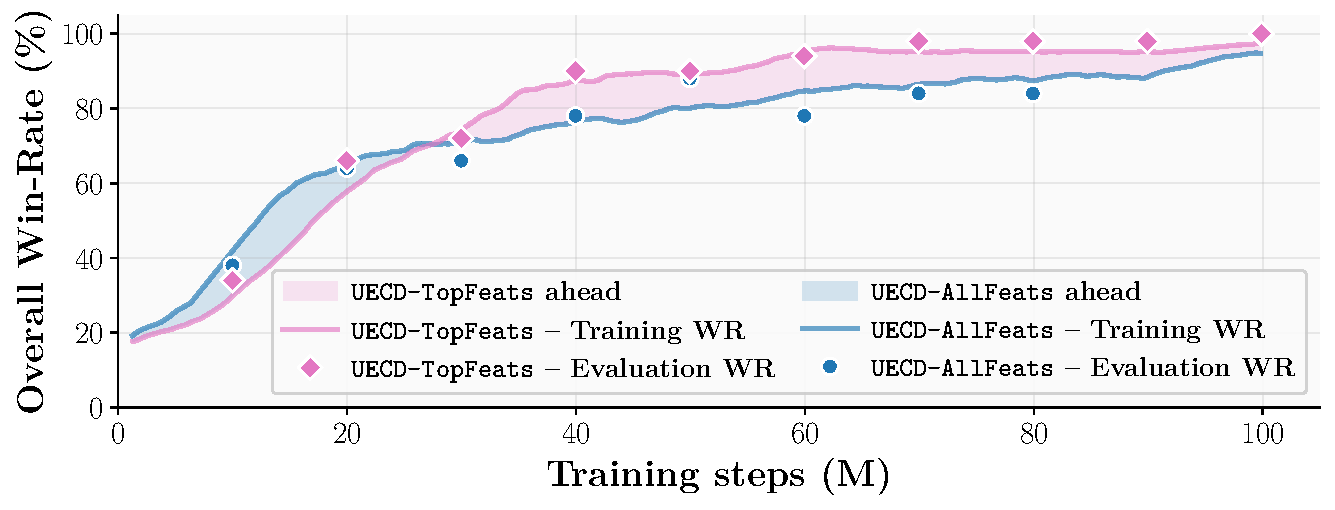
\includegraphics[width=0.81\columnwidth]{figures/best_vs_stier_100M.pdf}
\caption{\textbf{Training Curves:} WRs of \code{UECD-TopFeats} vs \code{UECD-AllFeats}.}
\label{fig:top_feats_vs_all_feats}
\end{figure}

Fig.~\ref{fig:top_feats_vs_all_feats} validates the top-$4$ cutoff: with $40$\% less compute, \code{UECD-TopFeats} pulls ahead of \code{UECD-AllFeats} on overall pool WR after ${\sim}20$--$30$\,M steps and converges to the same plateau, confirming that the extra eight features inflate training cost without lifting final performance.

\subsection{Final Training Run}
\label{sec:agent}

\subsubsection{\textbf{Rush Collapse Under Reward Anneal}}
\label{subsec:rush_collapse} 

Fig.~\ref{fig:reward_annealing} shows a training recipe (top-$4$ features, $300$\,M steps, shaped reward annealed linearly over [$90$\,M, $210$\,M], PFSP self-play) that collapses into a rush strategy as shaping fades. During the anneal, WR (top, green) climbs toward $100$\% while episode length (top, purple) drifts from ${\sim}1200$ to ${\sim}800$ frames. The crash happens in the final $10$\,M: WR drops to ${\sim}75$\% (recovering by $270$\,M) and episode length to ${\sim}300$ frames. Per-component returns (bottom) confirm the worker rush overfit: only \emph{WinDrawLoss} keeps rising, while \emph{ProduceBarracks} and \emph{MilitaryProduction} fall to zero, and \emph{ProduceWorker} drops from ${\sim}13.0$ to ${\sim}3.0$. This discount-induced shortcut is the optimal policy. Under terminal-only rewards, the RL objective $\mathbb{E}\bigl[\sum_{t=0}^{T} w_t^{\texttt{T}} R_t \gamma^t\bigr]$ collapses to $\mathbb{E}\bigl[w_T R_T \gamma^T\bigr]$, which for consistently-winning policies can be written as $w_T R_T \mathbb{E}\bigl[\gamma^T\bigr]$. This objective is maximized by minimizing $T$ since $\gamma < 1$, biasing fast wins over robust play. PPO's advantage-based updates inherit the same bias. With $\gamma{=}0.99$, shortening $T$ from $750$ to $300$ amplifies the terminal signal by $\gamma^{300}/\gamma^{750} \approx 90$. On unseen bots, WR collapses from $56.5$\% to $0$\% (TMA) and $70.4$\% to $1.5$\% (ObiBotKenobi) between $150$\,M and $300$\,M.

\begin{figure}[!tb]
\centering
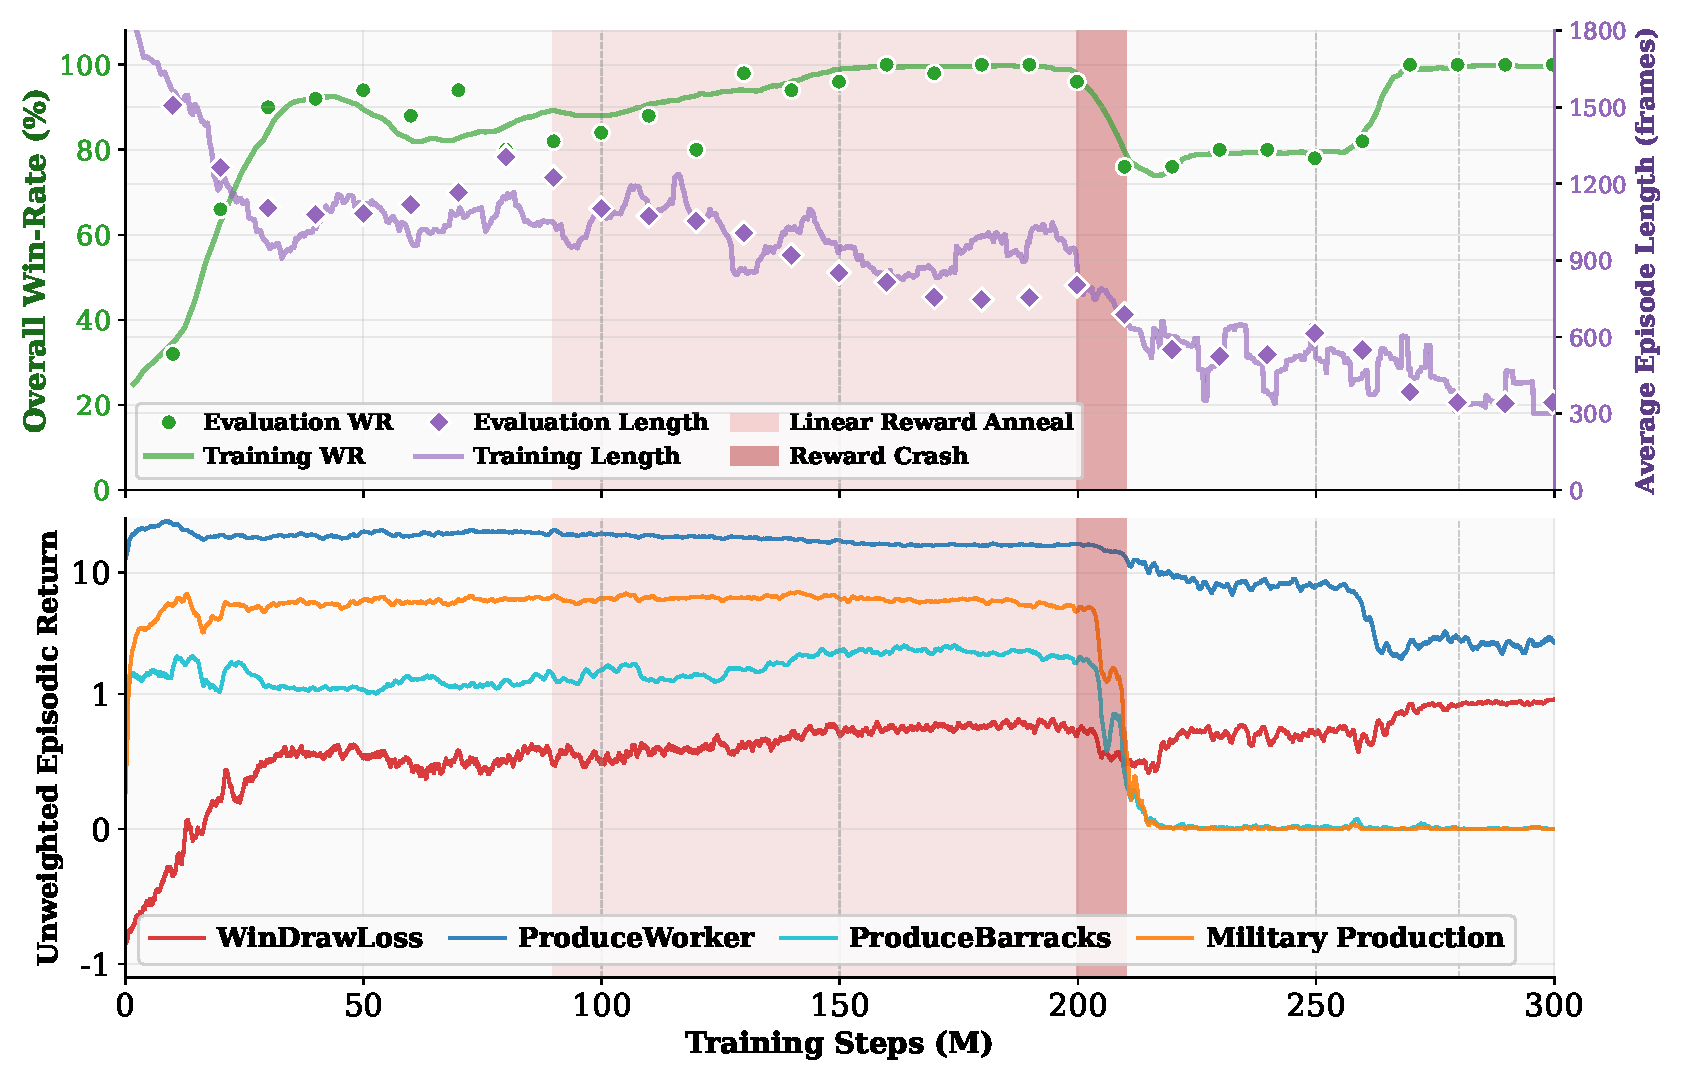
\includegraphics[width=0.86\columnwidth]{figures/rush_collapse.pdf}
\caption{\textbf{Rush Collapse:} WR (green) and episode length (purple); unweighted per-component returns (bottom); linear reward anneal (pink/red zones).}
\label{fig:reward_annealing}
\end{figure}

\subsubsection{\textbf{Opponent-Pool Fine-Tuning}}
\label{sec:finetuning}

To address this, training resumes from the $150$\,M checkpoint with shaped weight floored at $0.1$ rather than $0.0$, preserving a dense productive-action signal. Two fine-tuning phases face progressively stronger opponents. In Phase~$1$, TMA and ObiBotKenobi ($2$ envs each) replace the three weakest bots; self-play rises from $12$ to $16$ envs ($8$ latest / $8$ PFSP-hard; $24$ total envs). In Phase~$2$, RAISocketAI joins at $4$ envs, the rest at $1$ env each; self-play unchanged ($24$ bot envs). At $150$\,M, learning rate, entropy, and shaped weight start at ($5e{-}5$, $5e{-}3$, $1.0$); they anneal linearly to ($2e{-}5$, $2e{-}3$, $0.25$) at $240$\,M (end of Phase~$1$), and to ($9.5e{-}6$, $1.2e{-}3$, $0.10$) at $350$\,M (end of Phase~$2$).

The resulting agent, \code{UECD-Best}, is evaluated in Section~\ref{sec:tournament}. Training required \textbf{9.4 GPU-days} on an RTX $6000$ Ada ($48$ GB) across \textbf{350\,M steps}, roughly $7\times$ cheaper than RAISocketAI's $70$ GPU-days / $1.5$\,B steps over $8$ maps~\cite{goodfriendCompetitionWinningDeep2024}, trading breadth for depth through single-map specialization.

\section{Round-Robin Tournament}
\label{sec:tournament}

The $19$-agent tournament\footnote{\textbf{Supplementary Website:} $36$ recorded \code{UECD-Best} matchups, extended tournament game-theoretic metrics, source code, and CoG bots archive. Available at~\url{https://mathisdelsart.github.io/microrts-drl-uecd-website/}.} evaluates $15$ external agents (baselines, past CoG winners) and $4$ UECD checkpoints under the deterministic MicroRTS CoG protocol (Section~\ref{sec:setup-method}).

\code{UECD-Best} tops the standings with \textbf{174 points} (Fig.~\ref{fig:standings}; per-game scoring: $\text{Win}=+1$, $\text{Draw}=+0.5$, $\text{Loss}=+0$), ahead of RAISocketAI ($164$ points) and every intermediate \code{UECD} checkpoint. Rank-$1$ holds excluding these, ruling out a within-family bias. In head-to-head (Fig.~\ref{fig:h2h}), \code{UECD-Best} wins \textbf{100\%} against all except RAISocketAI ($90$\%) and POWorkerRush ($50$\%). However, under the stochastic protocol, \code{UECD-Best} wins $99.3$\% against POWorkerRush, resolving the deterministic-protocol artifact specific to this matchup. Against RAISocketAI, the WR drops to $65.7$\%, a narrower but still decisive margin. The improvement from \code{UECD-TopFeats} (131) to \code{UECD-Best} (174) confirms that two-phase fine-tuning bridges the gap to competitive play.

\begin{figure}[!t]
\centering
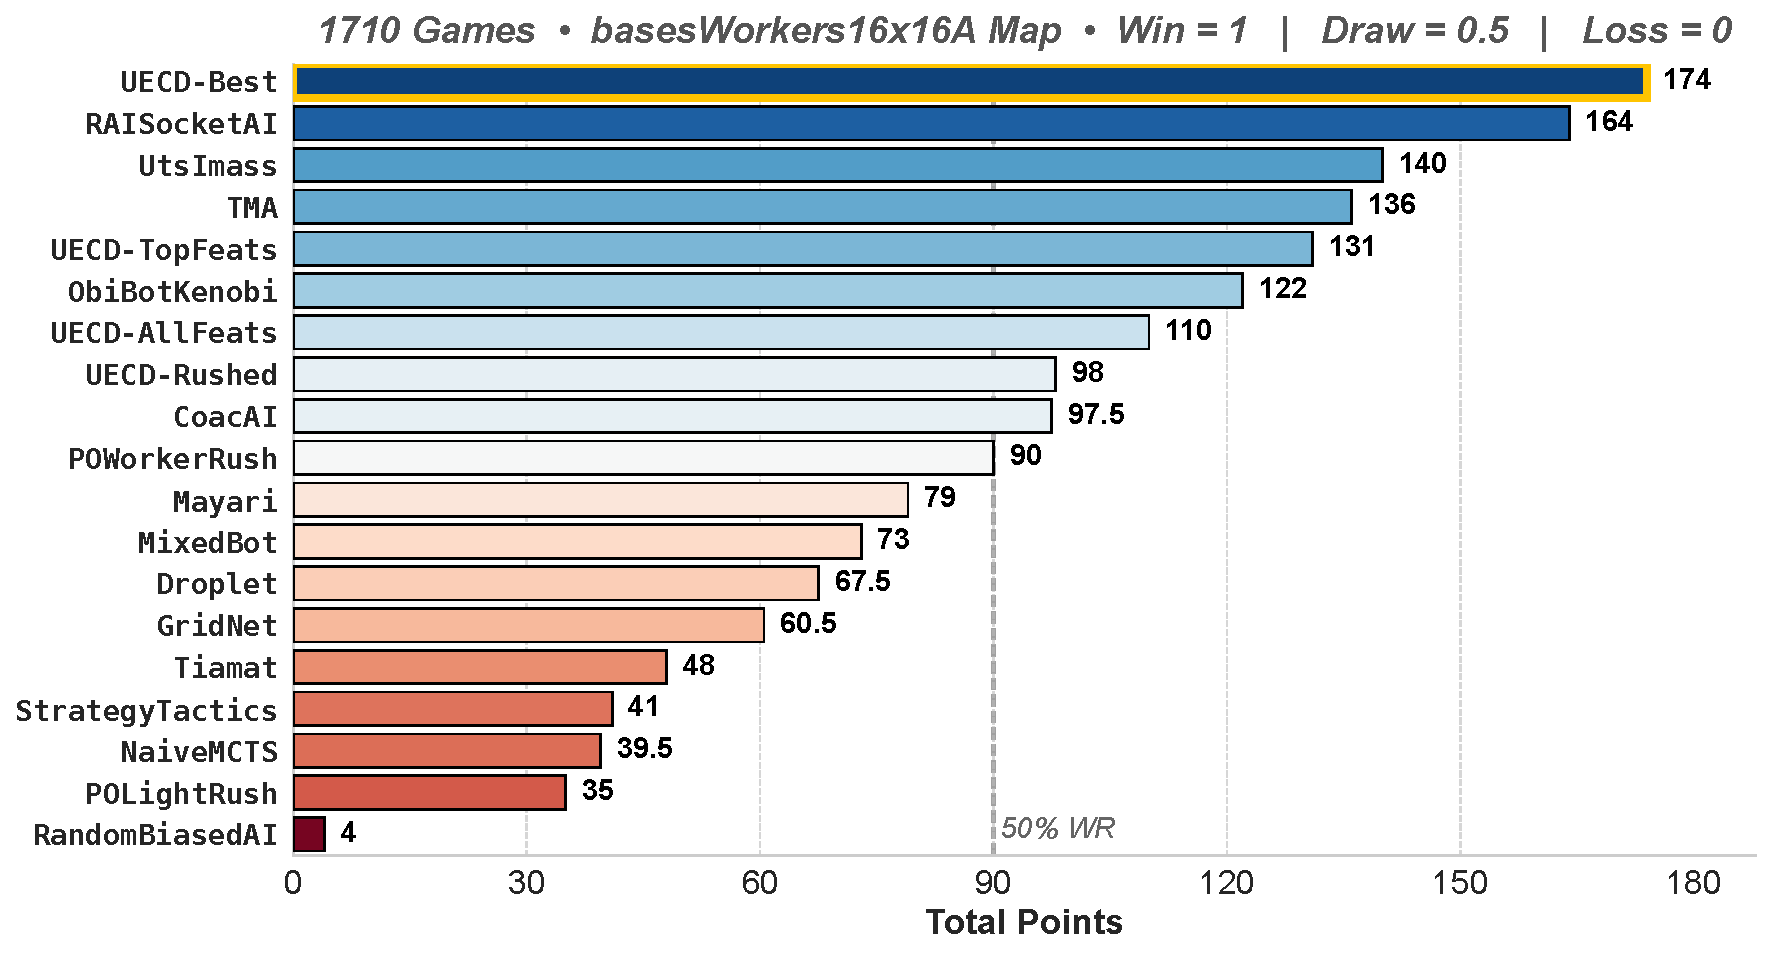
\includegraphics[width=0.92\columnwidth]{figures/final_standings.pdf}
\caption{\textbf{Final Tournament Standings:} $19$ agents ranked by total points.}
\label{fig:standings}
\end{figure}

\begin{figure}[!t]
\centering
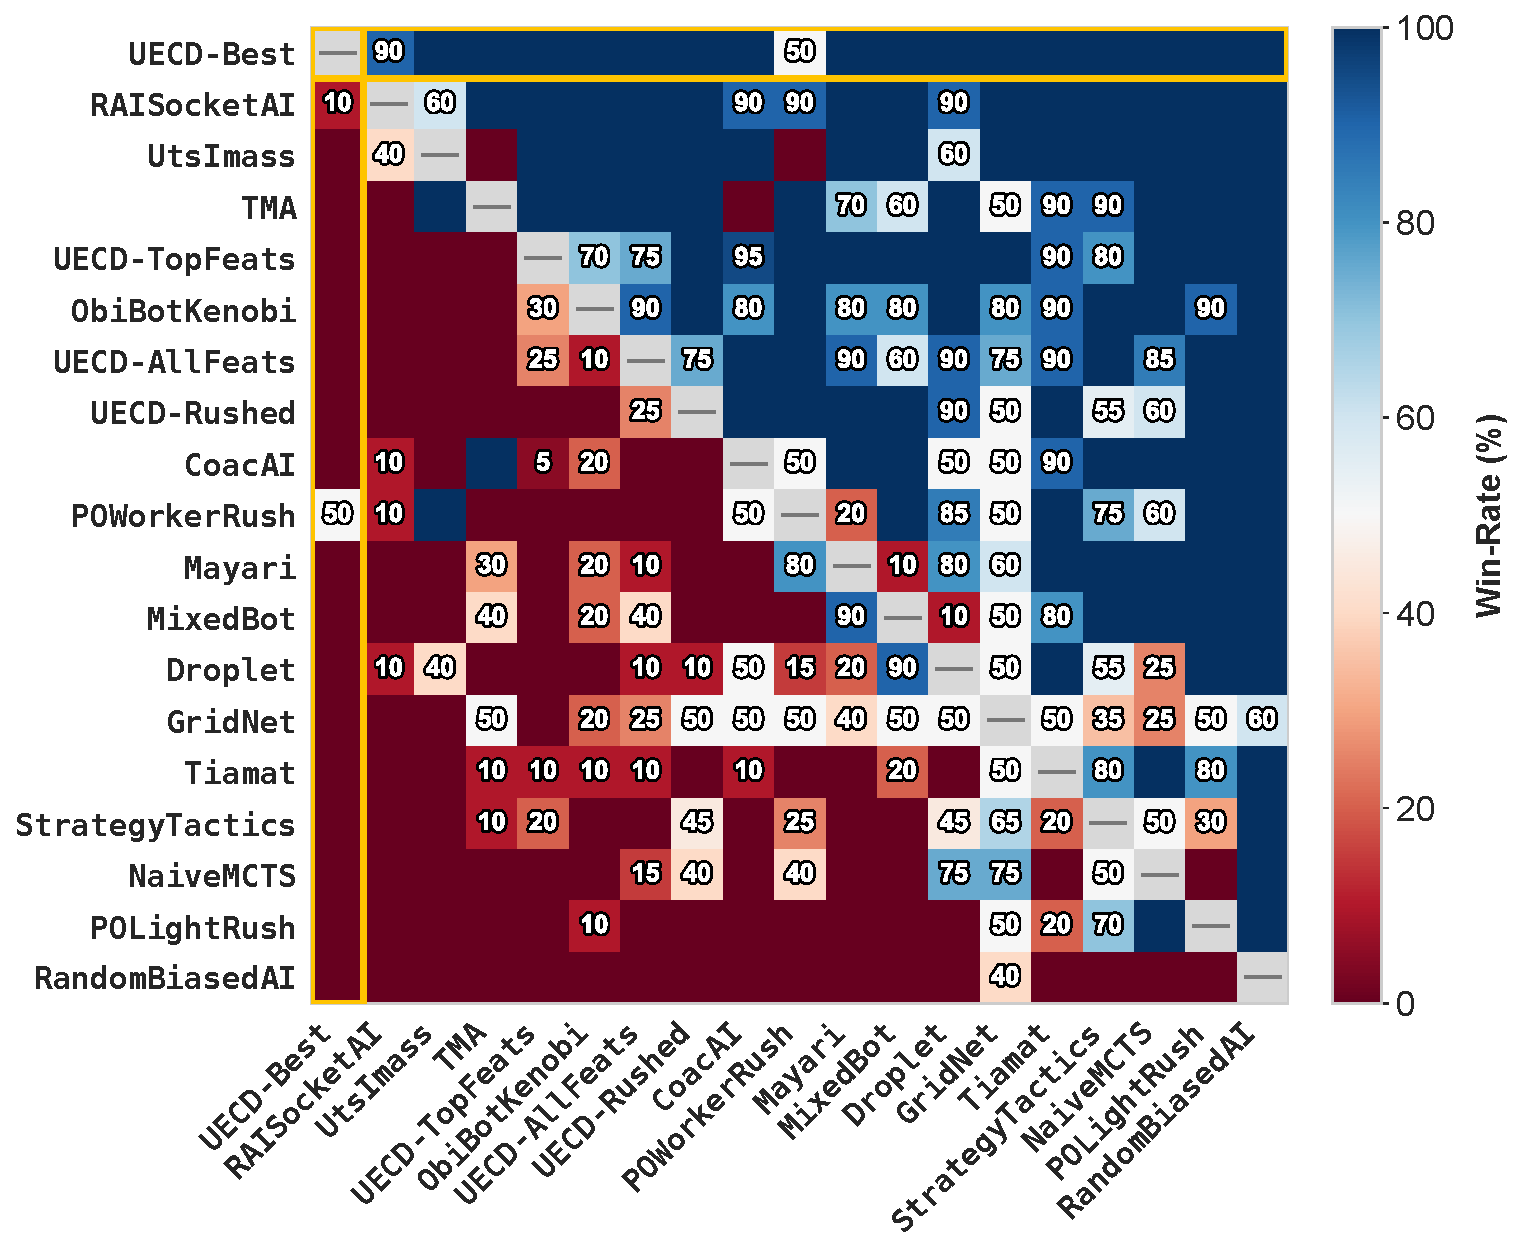
\includegraphics[width=0.88\columnwidth]{figures/h2h_matrix.pdf}
\caption{\textbf{Head-to-head WR Matrix:} $\texttt{WR}_{ij} = $ row agent $i$ vs column agent $j$}
\label{fig:h2h}
\end{figure}

\code{UECD-Best}'s replays reveal a narrow Ranged-only composition with tight micro-management. Game-theoretic analyses of the $19{\times}19$ WR matrix (Copeland, $\alpha$-Rank, and average regret) also rank \code{UECD-Best} first, with RAISocketAI second.

\section{Discussion and Limitations}
\label{sec:discussion}

\code{UECD-Best}'s single-map specialization isolates architectural and training contributions for clean per-component signal. Two distribution-shift probes assess the resulting out-of-distribution robustness (Fig.~\ref{fig:gen-probe}): a \textbf{\emph{layout} shift} (same size, different topology) and a \textbf{\emph{scale} shift} (same layout, larger size).
  
\begin{figure}[!tb]
\centering
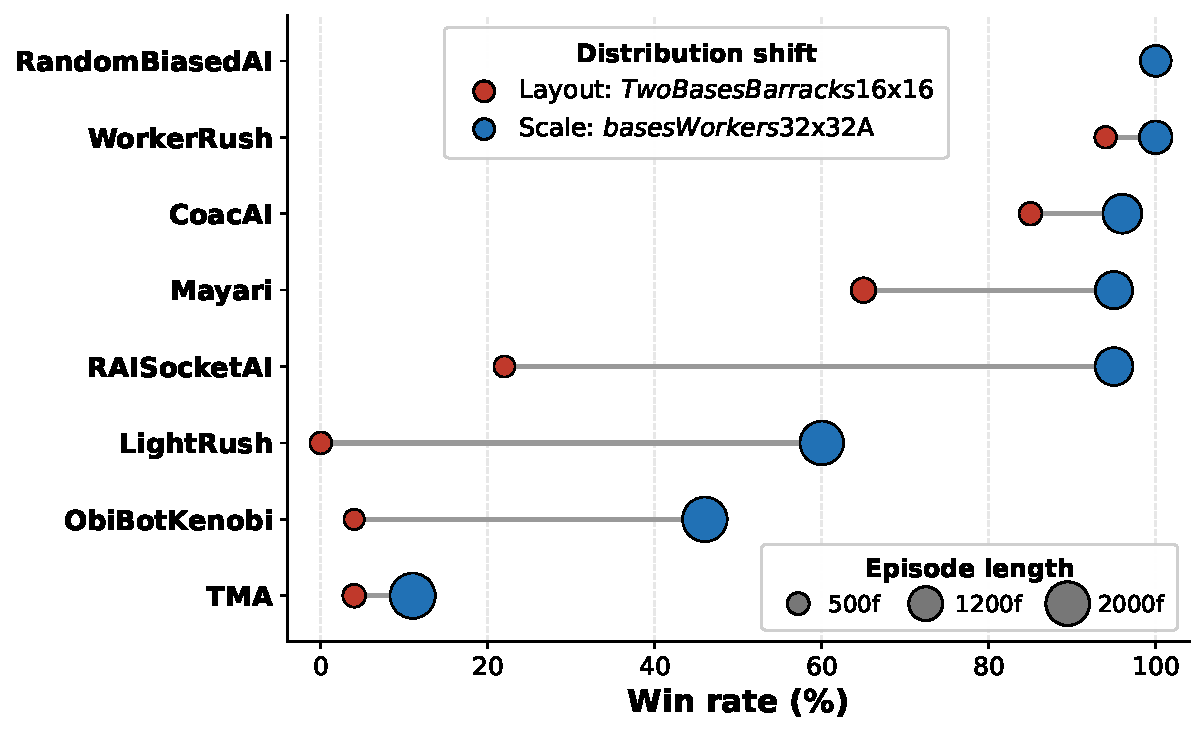
\includegraphics[width=0.87\columnwidth]{figures/generalization_probes.pdf}
\caption{\textbf{\code{UECD-Best} Generalization Probes:} \emph{layout} vs \emph{scale} shifts.}
\label{fig:gen-probe}
\end{figure}

The asymmetry is striking: scale-shift WR sits well above layout-shift WR for every opponent, and the gap widens against the strongest agents. Episode lengths, however, stay comparable across opponents in both shifts: the policy is not disoriented under distribution shift, just sub-optimal. The learned representation encodes map-specific geometric and topological priors rather than transferable strategic invariants. These findings only describe \code{UECD-Best} on shifts of its training map; performance under multi-map training or on unseen maps remains an open question (Section~\ref{sec:conclusion}).

\section{Conclusion and Future Work}
\label{sec:conclusion}

\code{UECD}'s explicit decomposition of RTS reasoning (spatial, relational, global; Section~\ref{sec:arch-ablation}) beats purely-spatial backbones at modest compute. The top-$4$ features (Section~\ref{sec:feat-ablation}) and training recipe (Section~\ref{sec:agent}) elevate \code{UECD-Best} to first place in the $19$-agent tournament on \emph{basesWorkers16x16A} (Section~\ref{sec:tournament}) with a \textbf{96.67\%} WR and a \textbf{9--1} head-to-head record against RAISocketAI on a \textbf{9.4} GPU-day budget.

The architecture is already size-agnostic; future work targets joint training on small maps ($\leq\!16{\times}16$) via padded environments and Prioritized Level Replay (PLR)~\cite{jiangPrioritizedLevelReplay2021}, then scaling to $64{\times}64$, where per-unit reasoning matters most.

\section*{Acknowledgment}

Computational resources have been provided by the Consortium des Équipements de Calcul Intensif (CÉCI), funded by the Fonds de la Recherche Scientifique de Belgique (F.R.S.-FNRS) under Grant No. 2.5020.11 and by the Walloon Region.

Anthropic's Claude (Opus 4) was used for English language polishing of the paper.


%% Bibliography

\hypersetup{urlcolor=black}
\begin{thebibliography}{10}
\providecommand{\url}[1]{#1}
\csname url@samestyle\endcsname
\providecommand{\newblock}{\relax}
\providecommand{\bibinfo}[2]{#2}
\providecommand{\BIBentrySTDinterwordspacing}{\spaceskip=0pt\relax}
\providecommand{\BIBentryALTinterwordstretchfactor}{4}
\providecommand{\BIBentryALTinterwordspacing}{\spaceskip=\fontdimen2\font plus
\BIBentryALTinterwordstretchfactor\fontdimen3\font minus
  \fontdimen4\font\relax}
\providecommand{\BIBforeignlanguage}[2]{{%
\expandafter\ifx\csname l@#1\endcsname\relax
\typeout{** WARNING: IEEEtran.bst: No hyphenation pattern has been}%
\typeout{** loaded for the language `#1'. Using the pattern for}%
\typeout{** the default language instead.}%
\else
\language=\csname l@#1\endcsname
\fi
#2}}
\providecommand{\BIBdecl}{\relax}
\BIBdecl
\renewcommand{\BIBentryALTinterwordstretchfactor}{4}

\bibitem{buroRTSChallenge2003}
M.~Buro, ``Real-time strategy games: A new {AI} research challenge,'' in
  \emph{Proc. Int. Joint Conf. Artif. Intell. ({IJCAI})}, 2003, pp. 1534--1535.

\bibitem{ontanonSurveyRealTimeStrategy2013}
S.~Onta{\~n}{\'o}n \emph{et~al.}, ``A survey of real-time strategy game {AI}
  research and competition in {StarCraft},'' \emph{{IEEE} Trans. Comput.
  Intell. {AI} Games}, vol.~5, no.~4, pp. 293--311, Dec. 2013.

\bibitem{vinyalsGrandmasterLevelStarCraft2019}
O.~Vinyals \emph{et~al.}, ``Grandmaster level in {StarCraft II} using
  multi-agent reinforcement learning,'' \emph{Nature}, vol. 575, no. 7782, pp.
  350--354, Nov. 2019.

\bibitem{ontanonCombinatorialMultiArmedBandit2013}
S.~Onta{\~n}{\'o}n, ``The combinatorial multi-armed bandit problem and its
  application to real-time strategy games,'' in \emph{Proc. {AAAI} Conf. Artif.
  Intell. Interact. Digit. Entertain. ({AIIDE})}, 2013, pp. 58--64.

\bibitem{ontanonFirstMicroRTSArtificial2018}
S.~Onta{\~n}{\'o}n, N.~A. Barriga, C.~R. Silva, R.~O. Moraes, and L.~H.~S.
  Lelis, ``The first {MicroRTS} artificial intelligence competition,''
  \emph{{AI} Mag.}, vol.~39, no.~1, pp. 75--83, Mar. 2018.

\bibitem{goodfriendCompetitionWinningDeep2024}
S.~Goodfriend, ``A competition winning deep reinforcement learning agent in
  {microRTS},'' in \emph{Proc. {IEEE} Conf. Games ({CoG})}, 2024, pp. 1--8.

\bibitem{ronnebergerUNetConvolutionalNetworks2015}
O.~Ronneberger, P.~Fischer, and T.~Brox, ``{U-Net}: Convolutional networks for
  biomedical image segmentation,'' in \emph{Proc. Med. Image Comput.
  Comput.-Assist. Interv. ({MICCAI})}, 2015, pp. 234--241.

\bibitem{wooCBAMConvolutionalBlock2018}
S.~Woo, J.~Park, J.-Y. Lee, and I.~S. Kweon, ``{CBAM}: Convolutional block
  attention module,'' in \emph{Proc. Eur. Conf. Comput. Vis. ({ECCV})}, 2018,
  pp. 3--19.

\bibitem{vaswaniAttentionAllYou2017}
A.~Vaswani \emph{et~al.}, ``Attention is all you need,'' in \emph{Proc. Adv.
  Neural Inf. Process. Syst. ({NeurIPS})}, 2017, pp. 5998--6008.

\bibitem{schulmanProximalPolicyOptimization2017}
\BIBentryALTinterwordspacing
J.~Schulman, F.~Wolski, P.~Dhariwal, A.~Radford, and O.~Klimov, ``Proximal
  policy optimization algorithms,'' 2017, arXiv:1707.06347. [Online].
  Available: \url{https://arxiv.org/abs/1707.06347}
\BIBentrySTDinterwordspacing

\bibitem{huangGym$m$RTSAffordableFull2021}
S.~Huang, S.~Onta{\~n}{\'o}n, C.~Bamford, and L.~Grela, ``Gym-{$\mu$RTS}:
  Toward affordable full game real-time strategy games research with deep
  reinforcement learning,'' in \emph{Proc. {IEEE} Conf. Games ({CoG})}, 2021,
  pp. 1--8.

\bibitem{huangCloserLookInvalid2022}
S.~Huang and S.~Onta{\~n}{\'o}n, ``A closer look at invalid action masking in
  policy gradient algorithms,'' in \emph{Proc. Int. {FLAIRS} Conf.}, 2022.

\bibitem{huSqueezeandExcitationNetworks2018}
J.~Hu, L.~Shen, and G.~Sun, ``Squeeze-and-excitation networks,'' in \emph{Proc.
  {IEEE/CVF} Conf. Comput. Vis. Pattern Recognit. ({CVPR})}, 2018, pp.
  7132--7141.

\bibitem{schulmanHighDimensionalContinuousControl2015}
J.~Schulman, P.~Moritz, S.~Levine, M.~Jordan, and P.~Abbeel, ``High-dimensional
  continuous control using generalized advantage estimation,'' in \emph{Proc.
  Int. Conf. Learn. Represent. ({ICLR})}, 2016.

\bibitem{espeholtIMPALAScalableDistributed2018}
L.~Espeholt \emph{et~al.}, ``{IMPALA}: Scalable distributed deep-{RL} with
  importance weighted actor-learner architectures,'' in \emph{Proc. Int. Conf.
  Mach. Learn. ({ICML})}, 2018, pp. 1407--1416.

\bibitem{manandharReinforcementActorcriticLearning2024}
S.~Manandhar and B.~Banerjee, ``Reinforcement actor-critic learning as a
  rehearsal in {MicroRTS},'' \emph{Knowl. Eng. Rev.}, vol.~39, p.~e6, Nov.
  2024.

\bibitem{jinPartialAdvantageEstimator2025}
Y.~Jin, X.~Song, G.~Slabaugh, and S.~Lucas, ``Partial advantage estimator for
  proximal policy optimization,'' \emph{{IEEE} Trans. Games}, vol.~17, no.~1,
  pp. 158--166, Mar. 2025.

\bibitem{vanhasseltLearningValuesMany2016}
H.~{van Hasselt}, A.~Guez, M.~Hessel, V.~Mnih, and D.~Silver, ``Learning values
  across many orders of magnitude,'' in \emph{Proc. Adv. Neural Inf. Process.
  Syst. ({NeurIPS})}, 2016, pp. 4287--4295.

\bibitem{hendrycksGaussianErrorLinear2016}
\BIBentryALTinterwordspacing
D.~Hendrycks and K.~Gimpel, ``Gaussian error linear units ({GELUs}),'' 2016,
  arXiv:1606.08415. [Online]. Available: \url{https://arxiv.org/abs/1606.08415}
\BIBentrySTDinterwordspacing

\bibitem{mnihHumanlevelControlDeep2015}
V.~Mnih \emph{et~al.}, ``Human-level control through deep reinforcement
  learning,'' \emph{Nature}, vol. 518, no. 7540, pp. 529--533, Feb. 2015.

\bibitem{heSpatialPyramidPooling2015}
K.~He, X.~Zhang, S.~Ren, and J.~Sun, ``Spatial pyramid pooling in deep
  convolutional networks for visual recognition,'' \emph{{IEEE} Trans. Pattern
  Anal. Mach. Intell.}, vol.~37, no.~9, pp. 1904--1916, Sep. 2015.

\bibitem{schaulPrioritizedExperienceReplay2015}
T.~Schaul, J.~Quan, I.~Antonoglou, and D.~Silver, ``Prioritized experience
  replay,'' in \emph{Proc. Int. Conf. Learn. Represent. ({ICLR})}, 2016.

\bibitem{jiangPrioritizedLevelReplay2021}
M.~Jiang, E.~Grefenstette, and T.~Rockt{\"a}schel, ``Prioritized level
  replay,'' in \emph{Proc. Int. Conf. Mach. Learn. ({ICML})}, 2021, pp.
  4940--4950.

\end{thebibliography}

\end{document}